\documentclass[10pt,a4paper]{article}
\usepackage[margin=2.25cm]{geometry}
\usepackage[T1]{fontenc}
\usepackage[utf8]{inputenc}
% Preserve the source dossiers' Unicode box drawings in their verbatim appendices.
\DeclareUnicodeCharacter{2500}{-}
\DeclareUnicodeCharacter{2502}{|}
\DeclareUnicodeCharacter{250C}{+}
\DeclareUnicodeCharacter{2510}{+}
\DeclareUnicodeCharacter{2514}{+}
\DeclareUnicodeCharacter{2518}{+}
\DeclareUnicodeCharacter{251C}{+}
\DeclareUnicodeCharacter{2524}{+}
\DeclareUnicodeCharacter{2550}{=}
\DeclareUnicodeCharacter{25BA}{>}
\usepackage{lmodern,microtype}
\usepackage{xcolor}
\usepackage{booktabs,tabularx,array,longtable}
\usepackage{amsmath,amssymb}
\usepackage{enumitem}
\usepackage{lscape}
\usepackage{tikz}
\usetikzlibrary{arrows.meta,positioning,fit,calc,shapes.geometric}
\usepackage{verbatim}
\usepackage{hyperref}
\definecolor{navy}{HTML}{123047}
\definecolor{teal}{HTML}{007C7A}
\definecolor{sky}{HTML}{DCEFF1}
\definecolor{orange}{HTML}{E67E22}
\definecolor{pale}{HTML}{F4F6F7}
\hypersetup{colorlinks=true,linkcolor=navy,citecolor=navy,urlcolor=navy,pdftitle={Semi-Humanoid Robotics: Comprehensive Literature Review}}
\setlength{\parindent}{1.2em}
\setlength{\parskip}{0.25em}
\renewcommand{\arraystretch}{1.16}
\newcolumntype{Y}{>{\raggedright\arraybackslash}X}
\newcommand{\evidence}[1]{\par\noindent\footnotesize\color{gray}\emph{Evidence basis: #1}\normalsize\par}

\begin{document}
\begin{center}
{\LARGE\bfseries Semi-Humanoid Robotics: A Comprehensive Literature Review of Platforms, Control, Embodied AI and Systems Integration\par}
\vspace{0.45em}
\small August 2026 \quad|\quad Scope: 2022--2026
\end{center}

\begin{abstract}
Semi-humanoid robotics joins a wheeled or tracked mobile base, a torso or lift, articulated arms, compliant end effectors and a sensorized interaction head. This report comprehensively consolidates two supplied literature reviews: an arXiv-oriented review of emerging open platforms, teleoperation and embodied-AI systems, and an OpenAlex-oriented review of peer-reviewed work on tactile sensing, task orchestration, human--robot interaction (HRI), digital twins and mobile manipulation. The reviewed evidence supports a systems research agenda in which the main challenge is not any isolated subsystem but the validated integration of modular mechanics, robust power and data interfaces, tactile contact, real-time safety, recovery logic, simulation and human-centred communication. The report separates source-reported findings from proposed design implications, retains all cited works and source-specific claims, and includes verbatim archival appendices of both supplied Markdown reports. Thus, no wording from the input dossiers is omitted from the report record.
\end{abstract}

\noindent\textbf{Keywords:} semi-humanoid robotics; mobile manipulation; bimanual teleoperation; tactile sensing; behavior trees; vision-language-action; digital twins; ROS~2; systems integration.

\section{Introduction}
Research in robotics is moving from isolated capabilities---fixed-base manipulation, navigation, or bipedal locomotion---toward integrated systems that must move, perceive, manipulate and safely interact with people. The supplied arXiv dossier characterises a semi-humanoid as a wheeled/track base, vertical torso or lift, dual 6--7 DoF arms, tactile or under-actuated grippers and an expressive sensor head. The supplied OpenAlex dossier complements this systems view with peer-reviewed foundations in compliant tactile sensing, behavior-tree reactivity, trajectory primitives, proactive HRI and human-centric digital twins.\cite{mobilealoha,yor,iovino,asad}

This report has two purposes. First, it provides a research-paper-form synthesis that preserves each substantive strand in the two dossiers. Second, it establishes a complete audit trail: Appendices~\ref{app:arxiv} and \ref{app:openalex} reproduce the supplied source documents verbatim. The appendices are archival evidence; the main text uses typeset equations, tables and editable TikZ diagrams rather than reproducing the sources' ASCII diagrams.

\section{Methodology and evidence protocol}
\subsection{Corpus and scope}
The corpus consists exclusively of the two user-provided Markdown reports. Both describe developments from 2022--2026. The arXiv review foregrounds emerging preprints, open platforms and implementation patterns. The OpenAlex review foregrounds peer-reviewed journals, conferences, DOIs and bibliometric claims. No new external search or independent source validation was undertaken for this synthesis.

\subsection{Synthesis procedure}
Each source was mapped into six common dimensions: platform architecture; manipulation and tactile hardware; teleoperation and whole-body control; task orchestration; multimodal AI and HRI; and simulation/digital twins. Repeated claims were reconciled, source-specific details were retained, and design recommendations were translated into falsifiable experimental artefacts. Citations refer to the works as listed in the supplied dossiers.

\subsection{Evidence limits}
The report uses ``reported'' for values, costs, citation counts, success rates and timing figures drawn from the source dossiers. Preprints offer timely system insight but should not be treated as peer-reviewed validation. Conversely, peer-reviewed component or survey literature does not independently demonstrate the complete proposed platform. Claims of ``gaps'' are therefore framed as gaps in the provided corpus or as integration opportunities, not absolute proof that no prior work exists.

\begin{figure}[ht]
\centering
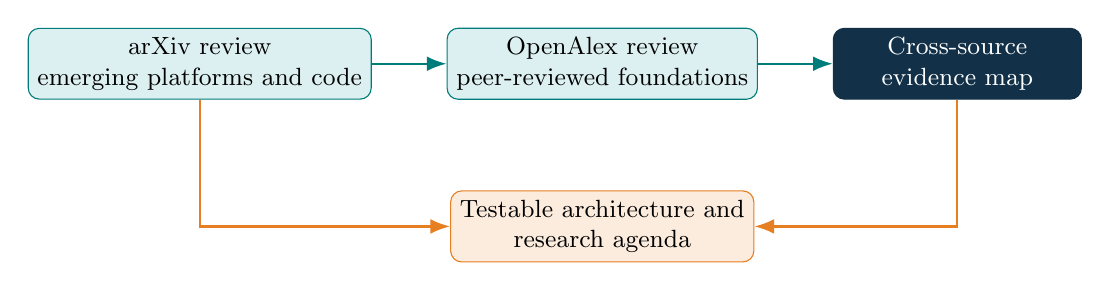
\begin{tikzpicture}[node distance=0.65cm and 0.95cm,every node/.style={font=\small,align=center},box/.style={draw=teal,fill=sky,rounded corners=4pt,minimum width=3.05cm,minimum height=0.8cm}]
\node[box] (pre) {arXiv review\\emerging platforms and code};
\node[box,right=of pre] (peer) {OpenAlex review\\peer-reviewed foundations};
\node[draw=navy,fill=navy,text=white,rounded corners=4pt,minimum width=3.15cm,minimum height=0.8cm,right=of peer] (map) {Cross-source\\evidence map};
\node[draw=orange,fill=orange!15,rounded corners=4pt,minimum width=3.6cm,minimum height=0.8cm,below=1.15cm of peer] (agenda) {Testable architecture and\\research agenda};
\draw[-{Latex[length=2.5mm]},thick,teal] (pre)--(peer);
\draw[-{Latex[length=2.5mm]},thick,teal] (peer)--(map);
\draw[-{Latex[length=2.5mm]},thick,orange] (map.south)|-(agenda.east);
\draw[-{Latex[length=2.5mm]},thick,orange] (pre.south)|-(agenda.west);
\end{tikzpicture}
\caption{Evidence protocol: emerging and peer-reviewed evidence are integrated, but their evidentiary roles remain distinct.}
\label{fig:method}
\end{figure}

\section{Taxonomy of semi-humanoid systems}
\subsection{Form factor and whole-body state}
For structured indoor environments, wheeled or omnidirectional mobility can reduce the cost and stability burden of bipedal locomotion while retaining mobile access to human-designed spaces. Mecanum or swerve bases provide planar $x$, $y$, $\theta$ motion and zero-radius turning; a telescopic lift substitutes vertical workspace expansion for leg kinematics. The whole-body state can be expressed as
\begin{equation}
\mathbf{q}=\begin{bmatrix}\mathbf{q}_{b}^{T} & q_{\ell} & \mathbf{q}_{L}^{T} & \mathbf{q}_{R}^{T}\end{bmatrix}^{T}, \qquad
\dot{\mathbf{x}}_e=\mathbf{J}(\mathbf{q})\dot{\mathbf{q}},
\label{eq:wbc}
\end{equation}
where $\mathbf{q}_b$ describes base motion, $q_{\ell}$ lift displacement, and $\mathbf{q}_L$, $\mathbf{q}_R$ arm joints. Whole-body inverse kinematics and MPC may coordinate these variables to preserve stability and reach.\cite{petrovic}

\begin{figure}[ht]
\centering
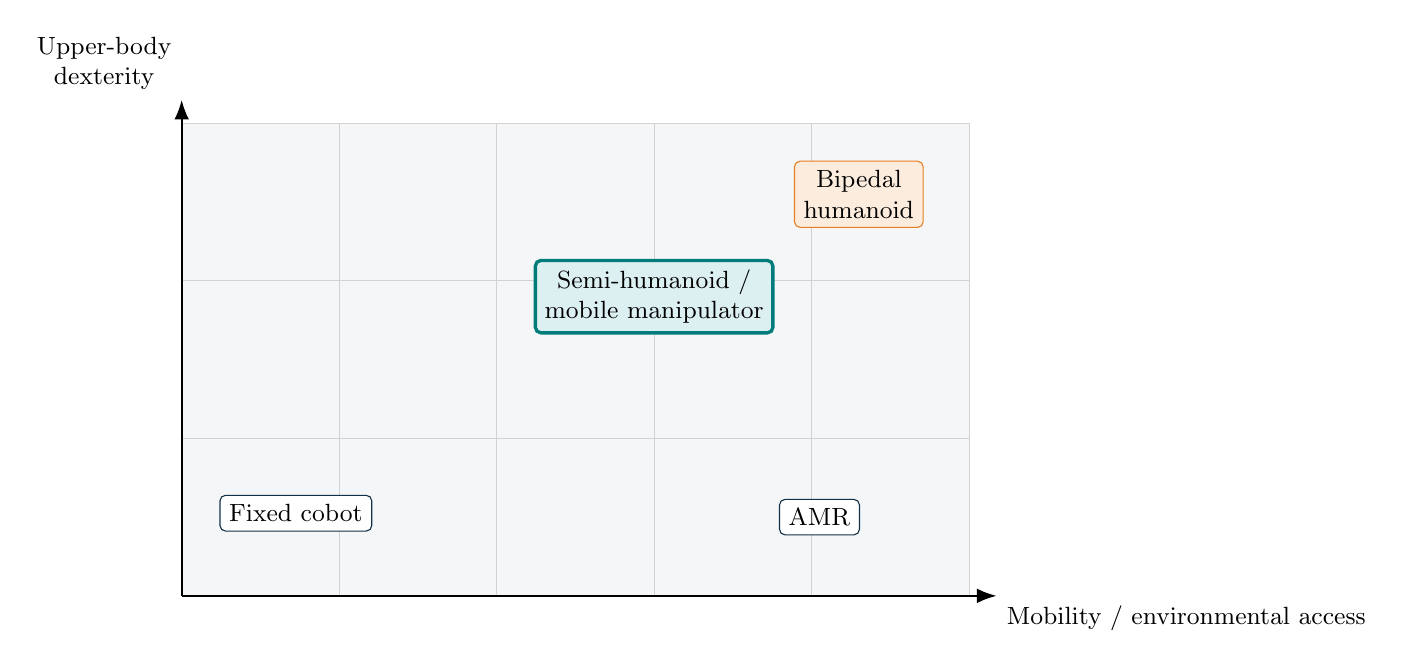
\begin{tikzpicture}[x=1cm,y=1cm,font=\small]
\fill[pale] (0,0) rectangle (10,6);
\draw[step=2cm,gray!35] (0,0) grid (10,6);
\draw[-{Latex[length=2.5mm]},thick] (0,0)--(10.35,0) node[below right]{Mobility / environmental access};
\draw[-{Latex[length=2.5mm]},thick] (0,0)--(0,6.3) node[above left,align=center]{Upper-body\\dexterity};
\node[draw=navy,fill=white,rounded corners=2pt] at (1.45,1.05) {Fixed cobot};
\node[draw=navy,fill=white,rounded corners=2pt] at (8.1,1.0) {AMR};
\node[draw=teal,fill=sky,very thick,rounded corners=2pt,align=center] at (6.0,3.8) {Semi-humanoid /\\mobile manipulator};
\node[draw=orange,fill=orange!15,rounded corners=2pt,align=center] at (8.6,5.1) {Bipedal\\humanoid};
\end{tikzpicture}
\caption{Design-space position of a semi-humanoid platform.}
\label{fig:taxonomy}
\end{figure}

\subsection{Platform benchmark and architectures}
Table~\ref{tab:platforms} retains the platform benchmark reported in the arXiv review. The benchmark mixes platform generations, openness models and cost-estimation bases; it is consequently a design reference rather than a controlled comparison.

\begin{table}[ht]
\centering\small
\caption{Platform taxonomy and reported comparison from the supplied arXiv review.}
\label{tab:platforms}
\begin{tabularx}{\textwidth}{@{}lYYrY@{}}
\toprule
Platform & Base and torso/reach & Arms, hands and HRI & Reported BOM & Hardware/software model \\
\midrule
YOR (NYU/Meta, 2026) & Omnidirectional; telescopic vertical lift & Dual 6-DoF arms, parallel grippers; dual RGB-D/head mount & <\$10k & Open source, COTS \\
Mobile ALOHA (Stanford, 2024) & Tracer wheeled chassis; fixed frame & Dual 6-DoF ViperX + leader arms; wrist/top RGB & \$\(\sim\)32k & Open hardware / software \\
Stretch 3 (Hello Robot) & Differential drive; telescopic column & 1-DoF arm + 2-DoF wrist gripper; ReSense RGB-D & \$\(\sim\)25k & Commercial, open API \\
TiAGO (PAL Robotics) & Differential/omni; motorised spine lift & Single/dual 7-DoF arms; pan-tilt head + microphone array & >\$90k & Commercial / proprietary \\
PR2 (Willow Garage) & Omnidirectional; telescopic spine & Dual 7-DoF arms; pan-tilt, stereo, LiDAR & >\$280k & Open source legacy baseline \\
Proposed platform & Modular omni/Mecanum; telescopic spine/active tilt & Dual modular 6--7 DoF; 3-DoF head, OAK-D, mic array & \$12--\$18k & Fully open integration standard \\
\bottomrule
\end{tabularx}
\evidence{Supplied arXiv review; cited platform works include \cite{yor,mobilealoha,stretch}.}
\end{table}

\section{Comprehensive technical synthesis}
\subsection{Pillar 1: modular mechatronics, mobility and bimanual platforms}
The arXiv dossier reports that bipedal locomotion can add unnecessary dynamic instability and cost in structured indoor settings. It highlights 3-DoF planar omnidirectional mobility, telescopic lift columns reaching floor to counter height, and low distal inertia through shoulder-mounted motors, Dyneema tendons and Bowden routing. It also identifies passive/adaptive end-effectors such as LEAP and BitoHand, with tendon networks and fingertip FSR arrays.\cite{yor,stretch}

The OpenAlex dossier complements these platform patterns with RSS 2023 low-cost bimanual hardware and imitation learning, reported as achieving over 90\% task success across fine-grained tasks such as bag zipping and bottle opening. It also includes a 2022 Precision Agriculture survey, which motivates wide-field RGB-D navigation plus wrist-mounted visual servoing in cluttered greenhouse picking.\cite{zhao,zhou}

\subsection{Pillar 2: tactile hands, soft-rigid mechanisms and contact sensing}
The scholarly corpus contains a soft, thumb-sized vision-based tactile sensor for continuous 3D force and sub-millimetre deformation estimation, a soft-rigid compliant-actuation review, an iontronic pressure-sensor reference and reports on tactile/soft hand concepts.\cite{sun,xavier,yang} Together, these works motivate a multi-scale sensing topology: a wrist 6-axis force/torque sensor for global load, fingertip FSR or pressure sensing for local contact, and visual/tactile imagery for deformation and slip cues. A generic contact-state estimator is
\begin{equation}
\hat{\mathbf{c}}=f_{\theta}\left(\mathbf{F}_{\mathrm{wrist}},\mathbf{p}_{\mathrm{finger}},\mathbf{I}_{\mathrm{tactile}},\mathbf{I}_{\mathrm{vision}}\right).
\label{eq:contact}
\end{equation}
The input documents identify an unresolved integration issue: published systems rarely standardise a modular wrist-to-fingertip topology combining rigid F/T sensing with compliant silicone skins.

\subsection{Pillar 3: teleoperation, whole-body control, behavior trees and DMPs}
Mobile ALOHA and OmniH2O are identified as leader-follower/master-slave infrastructures for whole-body teleoperation and data capture.\cite{mobilealoha,omnih2o} The arXiv dossier also reports ROS~2 Humble/Jazzy, Zenoh and micro-ROS as an evolution toward low-latency middleware and embedded execution. The OpenAlex dossier adds the Behavior Tree survey and the DMP tutorial survey: BTs provide modularity, reactivity and fault recovery compared with conventional FSMs, while DMPs provide a mathematically grounded way to represent, adapt and scale demonstrated trajectories.\cite{iovino,saveriano}

The combined implication is a two-part control architecture: a task layer that selects, sequences and recovers skills, and a fast control layer that regulates motion and contact. Bimanual operations need explicit recovery nodes for partial slip, blocked paths, elevator/door interaction, object handover and safe retreat---an open library and evaluated benchmark are more valuable than a one-off task graph.

\subsection{Pillar 4: multimodal AI and expressive HRI}
The arXiv report lists OpenVLA and SLIM as open VLA/action-grounded model directions that translate language-conditioned visual information into end-effector action proposals.\cite{openvla,slim} It also records work on expressive robotic heads, gaze/attention, episodic memory and TDOA microphone-array localisation.\cite{moraes,aschenbrenner} The OpenAlex review provides a peer-reviewed HRI foundation: proactive, predictable collaboration depends on intention signalling, including head orientation, gaze and displays before physical movement.\cite{li}

The proposed 3-DoF pan-tilt-roll head with OAK-D stereo vision, four-microphone TDOA array and OLED face display is therefore an experimentally testable HRI hypothesis. It should be assessed using predictability, workload, trust, attention alignment and perceived safety metrics rather than asserted to improve interaction by default.

\subsection{Pillar 5: simulation, digital twins and sim-to-real}
The source documents name MuJoCo, Isaac Sim, OpenUSD, semantic 3D Gaussian Splatting and reinforcement learning as simulation and pre-training infrastructure.\cite{ou,asad,han} The OpenAlex review foregrounds human-centric industrial digital twins that join physical telemetry, scene graphs and synthetic data for monitoring and collision prediction. The stated limitation is tactile/deformable contact: rigid-body simulation may represent chassis and arm kinematics well but does not necessarily reproduce silicone skin deformation, FSR response or contact friction. A credible pipeline must quantify the discrepancy:
\begin{equation}
\epsilon_{\mathrm{sim2real}}=\frac{1}{N}\sum_{i=1}^{N}\left\|\mathbf{y}^{\mathrm{sim}}_i-\mathbf{y}^{\mathrm{real}}_i\right\|,
\end{equation}
for declared output variables $\mathbf{y}$ such as force, pose, slip classification or task success.

\begin{figure}[ht]
\centering
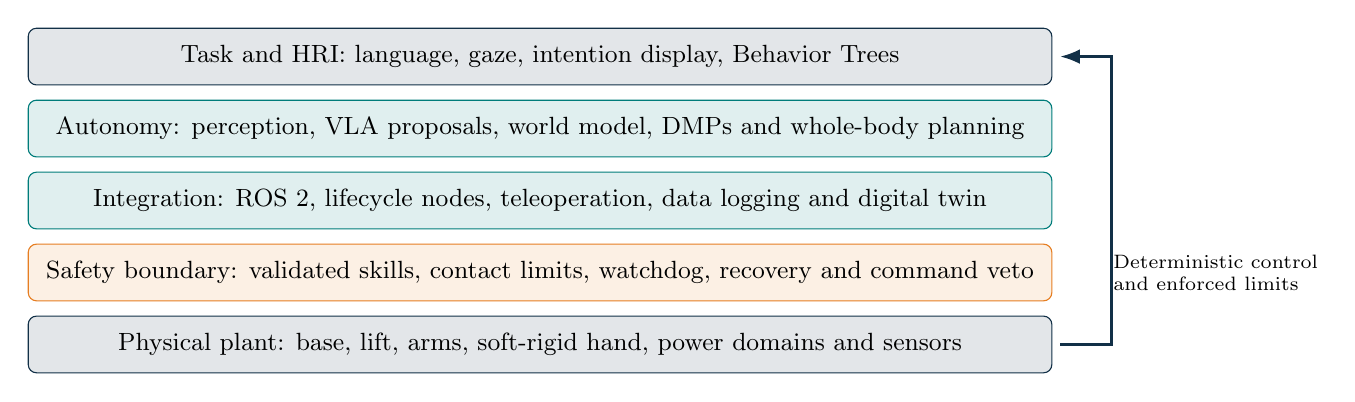
\begin{tikzpicture}[every node/.style={font=\small,align=center},layer/.style={draw=#1,fill=#1!12,rounded corners=3pt,minimum width=13cm,minimum height=0.72cm}]
\node[layer=navy] (hri) {Task and HRI: language, gaze, intention display, Behavior Trees};
\node[layer=teal,below=0.18cm of hri] (autonomy) {Autonomy: perception, VLA proposals, world model, DMPs and whole-body planning};
\node[layer=teal,below=0.18cm of autonomy] (integration) {Integration: ROS 2, lifecycle nodes, teleoperation, data logging and digital twin};
\node[layer=orange,below=0.18cm of integration] (safety) {Safety boundary: validated skills, contact limits, watchdog, recovery and command veto};
\node[layer=navy,below=0.18cm of safety] (plant) {Physical plant: base, lift, arms, soft-rigid hand, power domains and sensors};
\draw[-{Latex[length=2.5mm]},thick,navy] ($(plant.east)+(0.1,0)$)--++(0.65,0)|-($(hri.east)+(0.1,0)$);
\node[right=0.65cm of safety,font=\scriptsize,align=left] {Deterministic control\\and enforced limits};
\end{tikzpicture}
\caption{Integrated architecture implied by both dossiers. The orange boundary separates non-deterministic high-level proposals from real-time safety enforcement.}
\label{fig:stack}
\end{figure}

\section{Gap analysis and research contributions}
The two dossiers collectively identify ten gap statements. Five recur across both sources and five are source-specific elaborations. Table~\ref{tab:gaps} retains all of them while converting them into validation-oriented contributions.

\begin{longtable}{@{}p{0.23\textwidth}p{0.35\textwidth}p{0.34\textwidth}@{}}
\caption{Complete gap-to-contribution map from the supplied reviews.}\label{tab:gaps}\\
\toprule
Gap & Source-reported problem & Research-grade contribution and evidence \\
\midrule
\endfirsthead
\toprule
Gap & Source-reported problem & Research-grade contribution and evidence \\
\midrule
\endhead
Modular mechanical/electrical interfaces & Fixed, monolithic builds require manual rewiring and hard-coded reconfiguration when swapping arms, grippers or torso/base configurations. & ISO 9409-1-compatible quick-release pattern, blind-mate power/CAN, ROS~2 lifecycle discovery; report swap time, fault rate and configuration reproducibility. \\
VLM/VLA-to-motor latency and safety chasm & Source reports VLA inference at 5--10Hz versus contact-safe control at 1kHz; raw trajectory execution lacks a standard reflex veto. & Jetson cognitive layer at 10--30Hz; STM32/ESP32 micro-ROS layer at 1kHz; command-veto, contact and communication-loss fault-injection tests. \\
Galvanic clean/dirty power isolation & Back-EMF and high-current actuation can reset Jetson/camera logic; papers often omit PDB/schematic standards. & Isolated 24--48V motor and regulated 12/19V compute domains; transient, EMC, brownout and reset-resilience measurements. \\
Static/non-expressive low-cost heads & Mobile ALOHA/YOR-style static camera posts do not provide social cues, speaker tracking or integrated intention display. & Open 3-DoF head with OAK-D, four-mic TDOA and OLED face; compare HRI measures against a static-head baseline. \\
Cost, proprietary lock-in and fragility & Commercial platforms are reported at \$90k--\$280k while DIY platforms lack durability, documentation and replaceable-module standards. & Publish interface documents, BOM, calibration and service procedures; measure total build, repair and replication cost. \\
Rigid load-cell/soft-skin disconnect & Rigid 6-axis wrist sensors and soft skins are seldom integrated in one modular sensing topology. & Calibrated wrist-to-fingertip sensing stack; report contact-transition and load-sharing performance. \\
No standard bimanual BT recovery nodes & Existing BT implementations focus on single-arm or navigation cases. & Open BehaviorTree.CPP nodes for slip, obstruction, handover, door/elevator and retreat; report recovery success and time-to-recovery. \\
Deformable tactile sim-to-real gap & Isaac Sim-style rigid-body workflows do not fully model silicone deformation and fingertip FSR contact physics. & Instrumented contact benchmark, domain randomisation, hardware/simulation error curves and transfer protocol. \\
Agricultural/mobile-manipulator perception challenge & Cluttered unstructured picking needs broad navigation sensing plus wrist visual servoing. & Compare head, base and wrist sensor placement on clutter/occlusion tasks. \\
Data and demonstration cost & Real-world data collection is expensive, motivating teleoperation, synthetic data and policy pre-training. & Teleoperation dataset schema, quality controls, task coverage metrics and simulator-assisted augmentation study. \\
\bottomrule
\end{longtable}

\begin{figure}[ht]
\centering
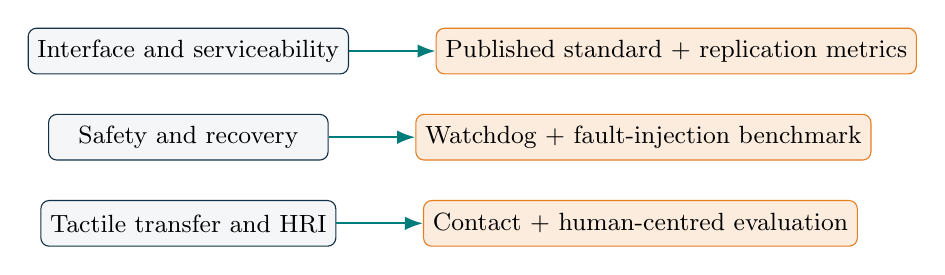
\begin{tikzpicture}[node distance=0.5cm and 1.1cm,every node/.style={font=\small,align=center},gap/.style={draw=navy,fill=pale,rounded corners=3pt,minimum width=3.55cm,minimum height=0.58cm},solution/.style={draw=orange,fill=orange!15,rounded corners=3pt,minimum width=4.55cm,minimum height=0.58cm}]
\node[gap] (g1) {Interface and serviceability}; \node[solution,right=of g1] (o1) {Published standard + replication metrics};
\node[gap,below=of g1] (g2) {Safety and recovery}; \node[solution,right=of g2] (o2) {Watchdog + fault-injection benchmark};
\node[gap,below=of g2] (g3) {Tactile transfer and HRI}; \node[solution,right=of g3] (o3) {Contact + human-centred evaluation};
\draw[-{Latex[length=2.3mm]},thick,teal] (g1)--(o1);
\draw[-{Latex[length=2.3mm]},thick,teal] (g2)--(o2);
\draw[-{Latex[length=2.3mm]},thick,teal] (g3)--(o3);
\end{tikzpicture}
\caption{A research contribution should convert the identified integration gaps into measurable artefacts and reproducible evidence.}
\end{figure}

\section{System design recommendations retained from the source dossiers}
\subsection{Hardware and interface recommendations}
The source recommendations call for a plug-and-play modular flange architecture: ISO~9409-1 mechanical patterns, combined power/CAN connectors and automatic ROS~2 lifecycle discovery. They propose modular SO-ARM100/Koch arms, LEAP/tactile hands, VESC motor controllers and a target BOM below \$15k (with a broader stated estimate of \$12k--\$18k). Proximal tendon actuation is recommended to lower distal inertia; soft-rigid five-finger hands combine wrist F/T sensing with fingertip FSRs.

\subsection{Compute, safety and power recommendations}
Both reports recommend a ``brain and spinal cord'' architecture: Jetson Orin with VLM/LLM and ROS~2 at approximately 10--30Hz, plus STM32/ESP32 micro-ROS at 1kHz for deterministic execution and impedance/reflex enforcement. At the actuator boundary, a generic impedance controller is
\begin{equation}
\mathbf{F}_{\mathrm{cmd}}=\mathbf{K}(\mathbf{x}_d-\mathbf{x})+\mathbf{D}(\dot{\mathbf{x}}_d-\dot{\mathbf{x}}),
\end{equation}
with independent limits for force, velocity, temperature and loss of communication. The supplied sources further recommend optocouplers/galvanic isolation and a dual-domain PDB separating dirty actuator power from clean compute/sensor power.

\subsection{Software, HRI and digital-twin recommendations}
The retained software proposal is ROS~2 with MoveIt~2/\texttt{ros2\_control}, BehaviorTree.CPP recovery nodes, teleoperation data capture, and an Isaac Sim OpenUSD SIL/vHIL pipeline with domain randomisation. The HRI proposal is a 3-DoF gimbal head integrating OAK-D stereo vision, a four-mic TDOA array and an OLED expression screen. The sources link these choices to project references including strawberry harvesting, FLEXIBOT, multi-floor navigation, WMS forklift operation, soft-rigid hand and empowered grasp projects; their complete mappings appear verbatim in Appendix~\ref{app:openalex}.

\section{Research methodology for validation}
\subsection{Experimental questions}
The combined literature suggests five answerable research questions: (RQ1) Does the interface standard reduce module-change time and integration errors? (RQ2) Does the enforced safety layer reject unsafe high-level commands within the specified control period? (RQ3) Does sensor fusion improve contact transition and grasp retention across compliant objects? (RQ4) Do bimanual recovery nodes improve completion and recovery time relative to a nominal-only tree? (RQ5) Does an active perception head improve specified HRI outcomes versus a static baseline?

\subsection{Metrics and reporting}
Report task success, productive-cycle time, intervention rate, recovery success, mean time to recovery, module swap time, availability, energy use, sensor/compute resets, contact-force tracking error and $\epsilon_{\mathrm{sim2real}}$. For HRI, predefine participant population, task, counterbalancing, questionnaire/scales and safety protocol. For all benchmarks, publish configurations, object sets, calibration, random seeds, failure cases and source code where possible.

\subsection{Threats to validity}
Reported prices and platform specifications are configuration-dependent. Teleoperation results may not generalise from demonstrations to autonomous execution. Simulation may conceal contact, latency and electrical effects. Small HRI studies may overstate generality. These threats reinforce the need for modular baselines, transparent failure reporting and on-hardware tests.

\section{Conclusion}
The supplied arXiv and OpenAlex reviews jointly describe a coherent field: mobile manipulation hardware is becoming more accessible; teleoperation and demonstrations are reducing data barriers; tactile sensing, BTs, DMPs and digital twins provide mature component foundations; and multimodal AI is expanding the space of high-level interaction. The strongest semi-humanoid research contribution is not a claim of general intelligence. It is a complete, measurable integration: modular and serviceable hardware, isolated power, explicit safety boundaries, calibrated contact sensing, recoverable task execution, validated sim-to-real transfer and human-centred communication.

\begin{thebibliography}{99}\small
\bibitem{yor} M. H. Anjaria et al., ``YOR: Your Own Mobile Manipulator for Generalizable Robotics,'' arXiv:2602.11150, 2026. \url{https://arxiv.org/abs/2602.11150}.
\bibitem{mobilealoha} Z. Fu, T. Z. Zhao, and C. Finn, ``Mobile ALOHA: Learning Bimanual Mobile Manipulation with Low-Cost Whole-Body Teleoperation,'' arXiv:2401.02117, 2024. \url{https://arxiv.org/abs/2401.02117}.
\bibitem{stretch} D. Honerkamp et al., ``Whole-Body Teleoperation for Mobile Manipulation at Zero Added Cost,'' arXiv:2409.15095, 2024. \url{https://arxiv.org/abs/2409.15095}.
\bibitem{omnih2o} T. He et al., ``OmniH2O: Universal and Dexterous Human-to-Humanoid Whole-Body Teleoperation and Learning,'' arXiv:2406.08858, 2024. \url{https://arxiv.org/abs/2406.08858}.
\bibitem{petrovic} G. R. Petrovi\'c and J. Mattila, ``Analytic Solutions for Wheeled Mobile Manipulator Supporting Forces,'' arXiv:2202.10186, 2022. \url{https://arxiv.org/abs/2202.10186}.
\bibitem{openvla} M. Molinari et al., ``Emergent World Representations in OpenVLA,'' arXiv:2509.24559, 2025. \url{https://arxiv.org/abs/2509.24559}.
\bibitem{slim} J. Wang et al., ``SLIM-0.5B: Learning Action-Grounded Predictive Latents for Robot Manipulation,'' arXiv:2608.09771, 2026. \url{https://arxiv.org/abs/2608.09771}.
\bibitem{moraes} P. Moraes et al., ``Hybrid Attention Estimation Pipeline for Adaptive HRI Using an Expressive Robotic Head,'' arXiv:2608.00284, 2026. \url{https://arxiv.org/abs/2608.00284}.
\bibitem{aschenbrenner} S. Aschenbrenner et al., ``Personalized Episodic Memory for the Humanoid Robot Head Kim,'' arXiv:2607.24190, 2026. \url{https://arxiv.org/abs/2607.24190}.
\bibitem{ou} H. Ou et al., ``Embodied Multimodal Grounding for Open-Vocabulary Mobile Manipulation via Semantic 3D Gaussian Splatting,'' arXiv:2608.10756, 2026. \url{https://arxiv.org/abs/2608.10756}.
\bibitem{zhao} T. Z. Zhao, V. Kumar, and S. Levine, ``Learning Fine-Grained Bimanual Manipulation with Low-Cost Hardware,'' RSS, 2023. DOI: \url{https://doi.org/10.15607/rss.2023.xix.016}.
\bibitem{sun} H. Sun, K. J. Kuchenbecker, and G. Martius, ``A Soft Thumb-Sized Vision-Based Sensor with Accurate All-Round Force Perception,'' \emph{Nature Machine Intelligence}, 2022. DOI: \url{https://doi.org/10.1038/s42256-021-00439-3}.
\bibitem{xavier} M. S. Xavier, C. Tawk, and A. Zolfagharian, ``Soft Pneumatic Actuators: A Review,'' \emph{IEEE Access}, 2022. DOI: \url{https://doi.org/10.1109/access.2022.3179589}.
\bibitem{iovino} M. Iovino et al., ``A Survey of Behavior Trees in Robotics and AI,'' \emph{Robotics and Autonomous Systems}, 2022. DOI: \url{https://doi.org/10.1016/j.robot.2022.104096}.
\bibitem{saveriano} M. Saveriano, F. J. Abu-Dakka, and A. Kramberger, ``Dynamic Movement Primitives in Robotics: A Tutorial Survey,'' \emph{IJRR}, 2023. DOI: \url{https://doi.org/10.1177/02783649231201196}.
\bibitem{li} S. Li, P. Zheng, and S. Liu, ``Proactive Human--Robot Collaboration,'' \emph{Robotics and Computer-Integrated Manufacturing}, 2022. DOI: \url{https://doi.org/10.1016/j.rcim.2022.102510}.
\bibitem{zhou} H. Zhou, X. Wang, and W. Au, ``Intelligent Robots for Fruit Harvesting: Recent Developments and Future Challenges,'' \emph{Precision Agriculture}, 2022. DOI: \url{https://doi.org/10.1007/s11119-022-09913-3}.
\bibitem{asad} U. Asad, M. Khan, and A. Khalid, ``Human-Centric Digital Twins in Industry,'' \emph{Sensors}, 2023. DOI: \url{https://doi.org/10.3390/s23083938}.
\bibitem{han} D. Han, B. Mulyana, and V. Stankovi\'c, ``A Survey on Deep Reinforcement Learning Algorithms for Robotic Manipulation,'' \emph{Sensors}, 2023. DOI: \url{https://doi.org/10.3390/s23073762}.
\bibitem{yang} R. Yang, A. Dutta, and B. Li, ``Iontronic Pressure Sensor with High Sensitivity over Ultra-Broad Linear Range,'' \emph{Nature Communications}, 2023. DOI: \url{https://doi.org/10.1038/s41467-023-38274-2}.
\end{thebibliography}

\end{document}
